The main mechanism that we needed was a way of intercepting system and library calls that an application makes in order to control the value returned. We needed a method that would be invisible and non-disruptive to the application being tested. Furthermore, it needed to be fine grained enough so that only calls from the  application being tested would be intercepted.

\subsection{LD\_PRELOAD} \label{ld_preload}
We intercepted system and library calls via the \texttt{LD\_PRELOAD} environment variable. Using \texttt{LD\_PRELOAD} a user can specify a shared library object that is loaded before any others at dynamic linking time. Importantly, functions within this shared library take precedence over any other functions of the same name, even ones found in \texttt{libc} and other standard libraries. For each call we wanted to test, we created a shared library object that contained a single wrapper function with the name of the call of interest. This wrapper would return an error value with probability $p$ or call the real version of the function to allow the application to continue as usual. A visual representation of this mechanism is given in figure \ref{fig:ld_preload}.

We used a probabilistic approach in order to test all the calls to a given function within an application. If the error values were returned deterministically, then only the first call to the function would be intercepted. The probability of an error being returned had to adjusted depending on the application and the call under testing. Some calls (especially ones related to resource allocation) were called many times within an application, requiring a lower probability, while others were called only a handful of times, requiring a higher probability. We used values from as low as 1\% to as high as 50\%.

\begin{figure}
  \centering
	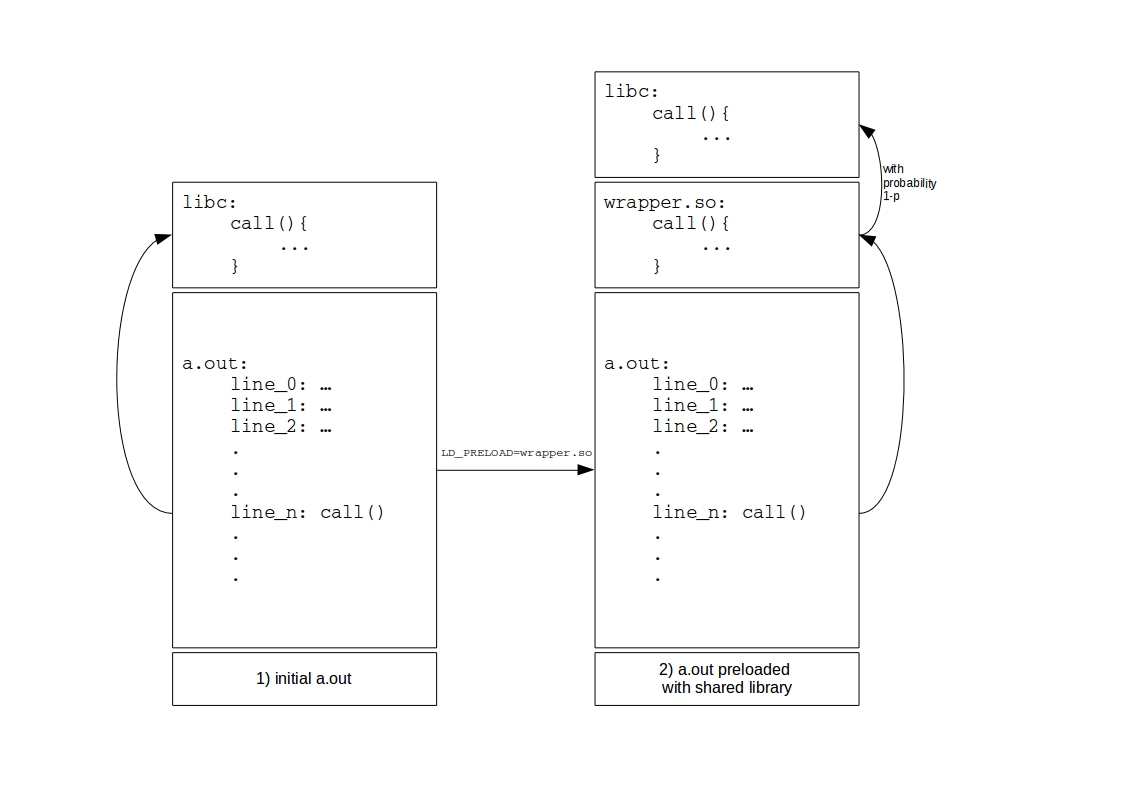
\includegraphics[width=0.8\textwidth]{ldpreload_fig}
	\caption{Library interposition allows for system and library calls to be overriden at runtime without recompilation or modification of the binary.}
  \label{fig:ld_preload}
\end{figure}

Calling the original function from within the wrapper is slightly trickier than one might expect. We couldn't simply call the function normally from the wrapper since it would lead to infinite recursion. To break this recursion, we used the \texttt{dlsym} function. \texttt{Dlsym} scans through dynamically loaded libraries looking for the function handle (that is, the address) of a function named as an argument. We can then use the function handle that is returned in order to call the original version of the function. An example of such a wrapper is given in listing 1.

\begin{minipage}{\linewidth} %minipage so the code is split between two pages
	\lstinputlisting[caption=\texttt{malloc} wrapper, language=C,label={lst:wrapper_example}]{sample_wrapper.c}
\end{minipage}

\subsubsection{Benefits of LD\_PRELOAD}
\texttt{LD\_PRELOAD} affords a number of benefits to the developer. Primarily, it is extremely simple to work with, and therefore difficult to get wrong: just set an environment variable and run the binary. We took this approach in order to test a greater number of calls and utilities as quickly as possible, but given more time may have opted to use binary rewriting. Furthermore, this method enables the interception of calls many levels deep in the stack, even in other dynamically linked libraries. We perceive this to be a benefit, as programs which depend on shared libraries are taking on the risk that those libraries are written incorrectly.

\subsubsection{Limitations of LD\_PRELOAD}
However there are several limitations to this method. Most significantly, applications that use statically linked libraries bypass our wrappers completely. Fortunately, we never encountered any applications that used static linking. If we wanted to expand coverage to programs that did use static linking we would need to use a binary rewriting tool as used by Miller et al. \cite{bart} or a dynamic instrumentation tool such as DynInst \cite{dyninst}.

Another limitation to our method is that it is Linux-specific. \texttt{LD\_PRELOAD} is found on many Linux distributions and some other UNIX systems, such as BSD \cite{bsd}. There are equivalents found on other popular systems such as the \texttt{AppInit\_DLLs} registry value on Windows \cite{dll} and the \texttt{DYLD\_INSERT\_LIBRARIES} environment variable on macOS \cite{macos}. We feel confident that our method could be applied to applications on these systems, but our current implementation is not portable.


